\def\CTeXPreproc{Created by ctex v0.2.9, don't edit!}
%\documentclass{beamer}
\documentclass[%handout,
xcolor=pdftex]{beamer}
\mode<presentation> {
  \usetheme{Warsaw}
  \setbeamercovered{transparent}
}
\let\Tiny=\tiny
\usetheme{Singapore}
\usecolortheme{dolphin}
\usepackage{amsmath}
\usepackage{textcomp}
\usepackage{amssymb}
\usepackage{amsthm}
\usepackage{graphicx}
\usepackage{color}
\usepackage{lipsum}
\usepackage{hyperref}
\usepackage{multirow}
\usepackage{bm}
%\setbeamertemplate{headline}{}
\setbeamertemplate{footline}[page number]
\newcommand\Fontvi{\fontsize{9pt}{8}\selectfont}
\newcommand\Fontvii{\fontsize{7pt}{8}\selectfont}
\newcommand{\backupbegin}{
   \newcounter{finalframe}
   \setcounter{finalframe}{\value{framenumber}}
}
\newcommand{\backupend}{
   \setcounter{framenumber}{\value{finalframe}}
}\newtheorem{proposition}{Proposition}
\title{Unit 14: Building ARIMA Models}
\author[STAT 5170: Applied Time Series, Unit 14]{Taylor R. Brown}
\institute{Department of Statistics, University of Virginia}
\date{Fall 2020}

\AtBeginSubsection[] {
  \begin{frame}<beamer>{Outline}
    \tableofcontents[currentsection,currentsubsection]
  \end{frame}
}

\begin{document}


\frame{\titlepage}


\begin{frame}
\frametitle{Readings for Unit 14}

Textbook chapter 3.6, 3.7.

\end{frame}



\begin{frame}
\frametitle{Last Unit}
\begin{enumerate}
\item Method of Moments Estimation
\item Maximum Likelihood Estimation
\end{enumerate}
\end{frame}

\begin{frame}
\frametitle{This Unit}
\begin{enumerate}
\item Integrated models for nonstationary data.
\item Building ARIMA models.
\end{enumerate}
\end{frame}


\begin{frame}
\frametitle{Motivation}

Thus far, we have assumed stationary ARMA models. We next consider ARIMA models, which basically consider differences of the observations to coerce stationarity. We then see how to go about building an ARIMA model using techniques we've looked at previously (and some new ones). These techniques are namely: exploratory data analysis (plots, transformations, identifying potential models), model estimation, model diagnostics, and model selection.

\end{frame}

\section{Integrated Models for Nonstationary Data}
\frame{\tableofcontents[currentsection]}

\begin{frame}
\frametitle{Integrated Models for Nonstationary Data}

Recall when we discussed exploratory data analysis and smoothing that we sometimes began with a model such as
 $$
 x_t=\mu_t + y_t
 $$
where $\mu_t$ was a non-stationary component (trend) and $y_t$ was a stationary zero-mean process.

\end{frame}

\begin{frame}
\frametitle{Integrated Models for Nonstationary Data}

If we assume $\mu_t$ was of the form $\beta_0+\beta_1 t$, then differencing yields
$$
\nabla x_t =\beta_1 + \nabla y_t
$$
which is a stationary time series.  In general if $\mu_t$ is a polynomial in $t$, such as $\beta_0+\beta_1 t+...+\beta_p t^d$, then
$$
\nabla^d x_t =d! \beta_d + \nabla^d y_t.
$$

\end{frame}

\begin{frame}
\frametitle{Integrated Models for Nonstationary Data}

A process is ARIMA$(p,d,q)$ if
$$
\nabla^d x_t=(1-B)^d x_t
$$
is ARMA$(p,q)$. Note: ARIMA models are sometimes called Box-Jenkins models.

\end{frame}

\begin{frame}
\frametitle{Integrated Models for Nonstationary Data}

If the mean of $\nabla^d x_t$ is zero then we can write the ARIMA model as
\begin{equation}
\phi(B)(1-B)^d x_t = \theta(B) w_t
\end{equation}
If a mean does exist then we can write
\begin{equation}
\phi(B)(1-B)^d x_t = \alpha + \theta(B) w_t
\end{equation}
where $\alpha=\mu(1-\phi_1- \cdots -\phi_p)$.

\end{frame}

\begin{frame}
\frametitle{Integrated Models for Nonstationary Data}

We usually use a first difference to account for a \textbf{linear} trend in the data. A second difference may be used to account for a \textbf{quadratic} trend in the data.

\end{frame}

\begin{frame}
\frametitle{Integrated Models for Nonstationary Data}

Recall that differencing can sometimes introduce more \textbf{dependence} in the data. Let's assume that our data has the following model
$$
x_t =\beta_0+\beta_1 t + y_t
$$
where
$$
y_t=\phi_1 y_{t-1}+\phi_2 y_{t-2}+w_t.
$$

Consider $\nabla x_t=\beta_1+ \nabla y_t$.

\end{frame}

\begin{frame}
\frametitle{Integrated Models for Nonstationary Data}

Define
$$
z_t=\nabla y_t=y_t-y_{t-1}
$$
So,
$$
\nabla y_t=y_t-y_{t-1}=\phi_1 (y_{t-1}-y_{t-2})+\phi_2 (y_{t-2}-y_{t-3})+w_t-w_{t-1}
$$
which we could write as
$$
z_t=\phi_1 z_{t-1}+\phi_2 z_{t-2}+w_t-w_{t-1}
$$
which is ARMA(2,1). Notice that the original noise term $y_t$
is an AR(2).

\end{frame}

\section{Building ARIMA Models}
\frame{\tableofcontents[currentsection]}

\begin{frame}
\frametitle{ARIMA Models}

We'll explore some techniques for identifying and estimating non-seasonal ARIMA models, as well as how to analyze the residuals after a model is estimated. Recall that ARIMA models are specified as ARIMA(p,d,q).

\end{frame}

\begin{frame}
\frametitle{Elements of ARIMA Models}

\begin{itemize}
\item The elements in the ARIMA model are typically specified, in the following order: AR order, differencing, MA order.
\item If $d=0$, we may call the model an ARMA(p,q) model.
\item If $d=0$ and $q=0$, we have an AR(p) model.
\item If $d=0$ and $p=0$, we have an MA(q) model.
\end{itemize}

\end{frame}

\begin{frame}
\frametitle{Building ARIMA Models}

The main steps in building an ARIMA model are

\begin{itemize}
\item Exploratory data analysis (plots, transformations, identifying potential models).
\item Model estimation.
\item Model diagnostics.
\item Model selection.
\end{itemize}

\end{frame}

%\subsection{Exploratory Data Analysis}


\begin{frame}
\frametitle{Exploratory Data Analysis}

We typically look at

\begin{itemize}
\item the time series plot,
\item the ACF,
\item and the PACF
\end{itemize}

of the data. This step guides us to our choice for the elements of the ARIMA model, $p,d,q$.

\end{frame}

\begin{frame}
\frametitle{Exploratory Data Analysis: Time Series Plot}

We usually check for stationarity in a time series plot. Recall for stationarity, the plot should suggest the mean and the variance are constant. What we look out for in a time series plot:

\begin{itemize}
\item Trend (increasing, decreasing, quadratic).
\item Increasing variability.
\item Seasonality (talk about next unit).
\item Outliers.
\end{itemize}


\end{frame}

\begin{frame}
\frametitle{Exploratory Data Analysis: Time Series Plot}


We usually try to stabilize the variance first. If the variance appears to be increasing, we can try transforming the data, usually a log transform.

\end{frame}

\begin{frame}
\frametitle{Exploratory Data Analysis: Time Series Plot}

If there's a linear trend, we consider a first difference. A quadratic trend suggests a second difference. We rarely go beyond $d=2$, unless there is a contextual or scientific reason to do so. \\
\vspace{5mm}
As mentioned earlier, over-differencing can introduce unnecessary dependency in the model. \textbf{Smoothing techniques} may be used, where we analyze the smoothed data instead.

\end{frame}

\begin{frame}
\frametitle{Exploratory Data Analysis: ACF and PACF}

The ACF and PACF should be used together. Recall that

\begin{itemize}
\item AR(p) models have theoretical PACF with non-zero values for $h \leq p$, and zero values for $h>p$. The ACF should decay exponentially to zero.
\item MA(q) models have theoretical ACF with non-zero values for $h \leq q$, and zero values for $h>q$. The PACF should decay exponentially to zero.
\item ARMA(p,q) models have ACF and PACF that both decay exponentially to zero. The order will not be obvious. In such a case, we may just start off with $p,q = 1 \text{ or } 2$, and see what happens during model estimation and diagnostics.
\end{itemize}


\end{frame}

\begin{frame}
\frametitle{Exploratory Data Analysis: ACF and PACF}

\begin{itemize}
\item If the ACF and PACF decay slowly (do not decay exponentially), then the time series is likely to be not stationary (was differencing performed earlier?).
\item If all the autocorrelations are insignificant for $h \geq 1$, than the series is (possibly-shifted) white noise.
\item If all the autocorrelations are insignificant for $h \geq 1$ for a first difference, then we may have a \textbf{random walk}.
\end{itemize}


\end{frame}

%\subsection{Model Estimation}

\begin{frame}
\frametitle{Model Estimation}

After exploratory data analysis, you should have an idea (or ideas) about the values of $p,d,q$. We use computer software (e.g. R) to estimate the parameters. Maximum likelihood estimation is usually used.

\end{frame}

\begin{frame}
\frametitle{Model Estimation: Significance of Estimates}

For the estimated coefficients of the parameters, use the $t$ statistic

$$
t = \frac{\mbox{estimated coefficient}}{\mbox{s.e. of coefficient}}.
$$

If $|t| > t_{1 - \alpha/2, df}$, the estimated coefficient is significantly different from 0 at 0.05 significance level.

\end{frame}

%\subsection{Model Diagnostics}


\begin{frame}
\frametitle{Model Diagnostics}

For model diagnostics, we usually check the following:

\begin{itemize}
\item ACF of residuals.
\item Ljung-Box-Pierce statistic.
\item Plot of residuals against fitted values or time series of residuals.
\end{itemize}

If our model diagnostics are acceptable, we expect our residuals to behave like \textbf{white noise}. If something appears unreasonable, you might have to revise your thought at what the model might be.

\end{frame}

\begin{frame}
\frametitle{Model Diagnostics: ACF of Residuals}

If you have a good model, all estimated ACFs of residuals should be \textbf{insignificant}. If this isn't the case, you probably need to explore a different model.

\end{frame}


\begin{frame}
\frametitle{Model Diagnostics: Ljung-Box-Pierce Statistic}

Recall that for white noise, the sample autocorrelations are approximately independent and normally distributed with mean 0 and variance $\frac{1}{n}$. The Ljung-Box-Pierce Q-statistic takes into account the magnitudes of the sample autocorrelations as a whole.

\end{frame}

\begin{frame}
\frametitle{Model Diagnostics: Ljung-Box-Pierce Statistic}

The Ljung-Box-Pierce statistic is a function of accumulated sample autocorrelations, $\hat{\rho}(h)$, up to a specified time lag $H$. The Ljung-Box-Pierce Q-statistic is given by

\begin{equation} \label{eq:ljung}
Q(H) = n(n+2) \sum_{h=1}^H \frac{\hat{\rho}(h)^2}{n-h}.
\end{equation}

The choice of $H$ is somewhat arbitrary. In R, $H$ is 20.

\end{frame}

\begin{frame}
\frametitle{Model Diagnostics: Ljung-Box-Pierce Statistic}

Under the null hypothesis that the model fits the data adequately, $Q \sim \chi^2_{H-p-q}$ as $n \to \infty$. A large Q-statistic leads to the rejection of the null hypothesis, i.e. \textbf{model is not an adequate fit for the data}.


\end{frame}

\begin{frame}
\frametitle{Model Diagnostics: Residual Plot}

Using either a plot of residuals against fitted values, or a time series plot of the residuals, we check if the variance is constant. If the variance is not constant, you may need to transform the data.


\end{frame}

%\subsection{Model Selection}


\begin{frame}
\frametitle{Model Selection}

Sometimes you may have more than one set of values for $p,d,q$ from exploratory data analysis. To be thorough, you may want to investigate the model estimation and diagnostics for more than one model. If model diagnostics suggest more than one model works, here are some issues to keep in mind when comparing models:

\begin{itemize}
\item Simpler model.
\item Standard errors of forecasts.
\item AIC, AICc, BIC etc.
\end{itemize}


\end{frame}

\begin{frame}
\frametitle{Model Selection}

Two different ARIMA models can be nearly equivalent when converted to an infinite order MA model using the causal representation.

\end{frame}

\section{Worked Example}
\frame{\tableofcontents[currentsection]}

\begin{frame}
\frametitle{Worked Example: US GNP}

To tie everything in, we'll look at an example on how to build an ARIMA model. We will use data on US gross national product in billions of chained 1996 dollars. The observations are quarterly data from 1947 to 2002.

\end{frame}

\begin{frame}
\frametitle{Worked Example: Exploratory Data Analysis}

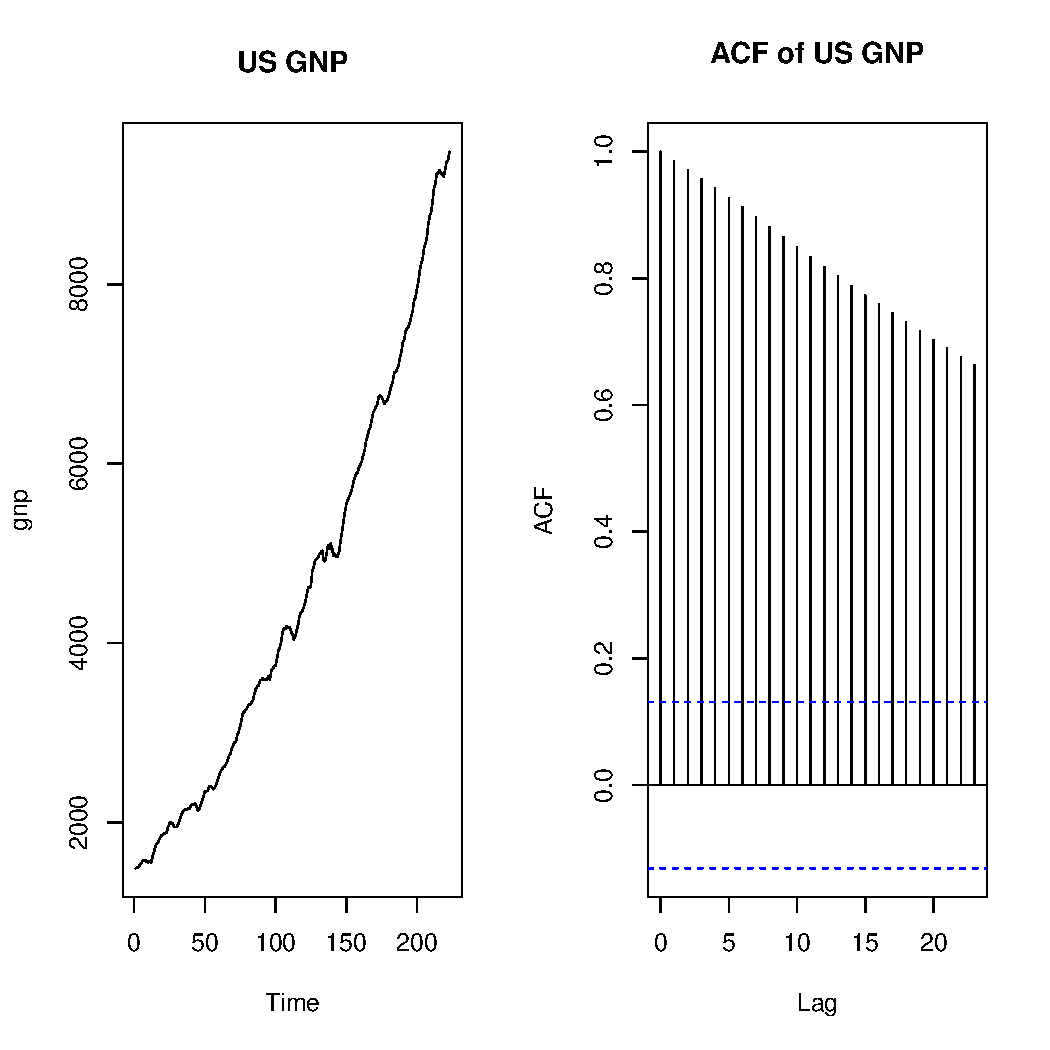
\includegraphics[width=100mm, height=60mm]{ts.pdf}

\textbf{Question}: Any comments on stationarity?

\end{frame}

\begin{frame}
\frametitle{Worked Example: Exploratory Data Analysis}

Let's look at growth rate, usually defined as $\nabla \log(x_t)$.

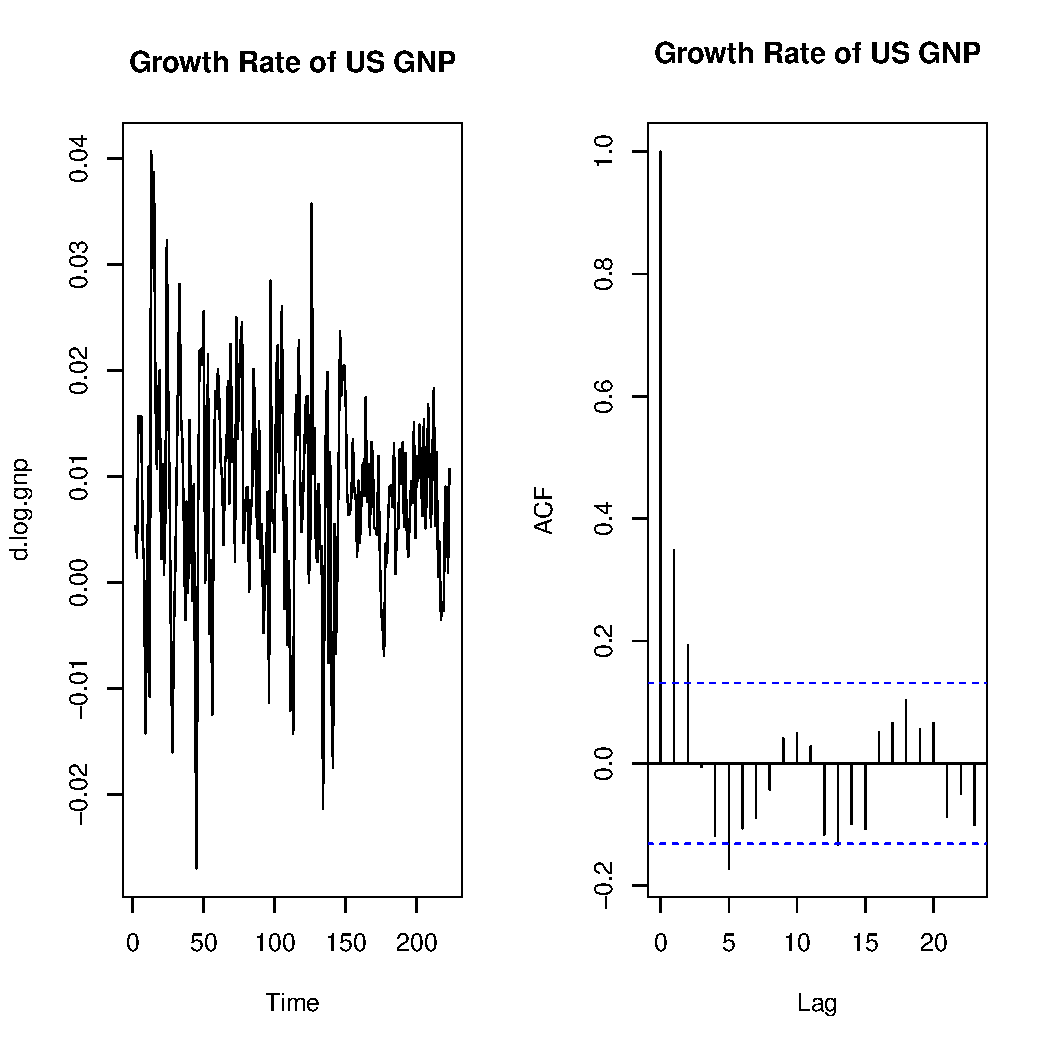
\includegraphics[width=100mm, height=50mm]{growth.pdf}

\textbf{Question}: Any comments on stationarity?

\end{frame}

\begin{frame}
\frametitle{Worked Example: Exploratory Data Analysis}

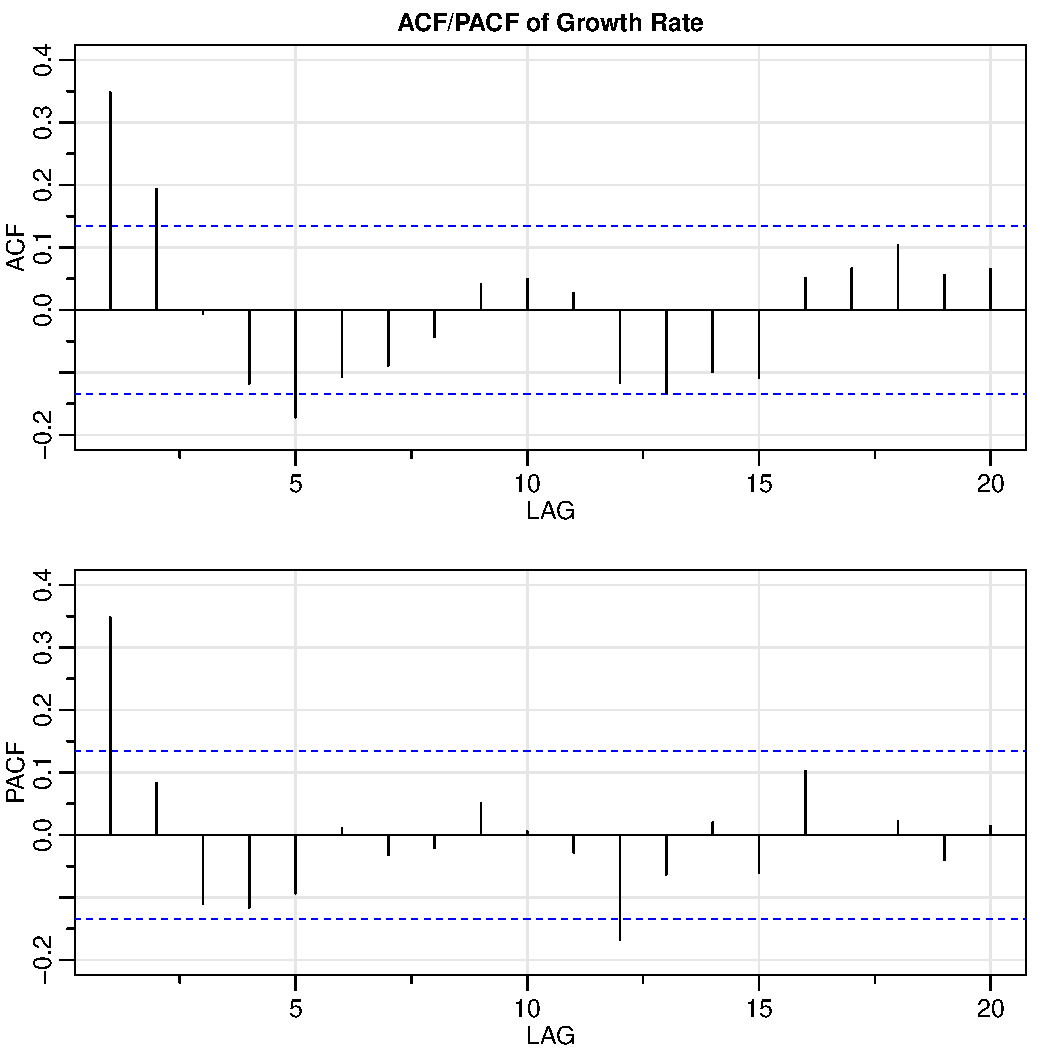
\includegraphics[width=100mm, height=60mm]{acf.pdf}

\textbf{Question}: What do you think for $p, q$?

\end{frame}

\begin{frame}[fragile]
\frametitle{Worked Example: Model Estimation}

Fit using \verb=sarima()= function in R.

\begin{verbatim}
      Estimate     SE t.value p.value
ar1     0.3467 0.0627  5.5255       0
xmean   0.0083 0.0010  8.5398       0
\end{verbatim}

\textbf{Question}: How to write this model?

\end{frame}

\begin{frame}[fragile]
\frametitle{Worked Example: Model Estimation}

Fit using \verb=sarima()= function in R.

\begin{verbatim}
      Estimate     SE t.value p.value
ma1     0.3028 0.0654  4.6272  0.0000
ma2     0.2035 0.0644  3.1594  0.0018
xmean   0.0083 0.0010  8.7178  0.0000
\end{verbatim}

\textbf{Question}: How to write this model?

\end{frame}

\begin{frame}
\frametitle{Worked Example: Model Diagnostics}

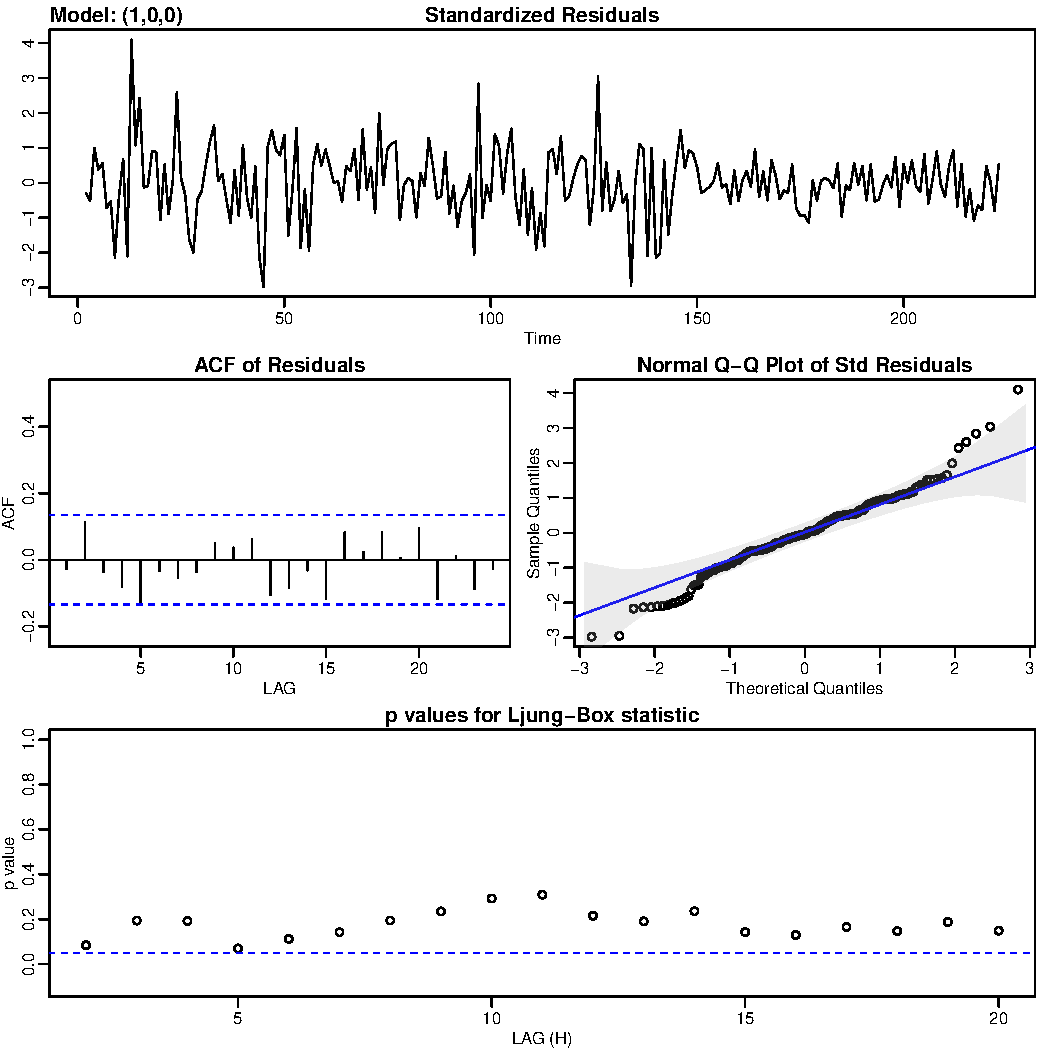
\includegraphics[width=100mm, height=60mm]{ar_diag.pdf}

Diagnostic plots for AR(1) model.

\end{frame}

\begin{frame}
\frametitle{Worked Example: Model Diagnostics}

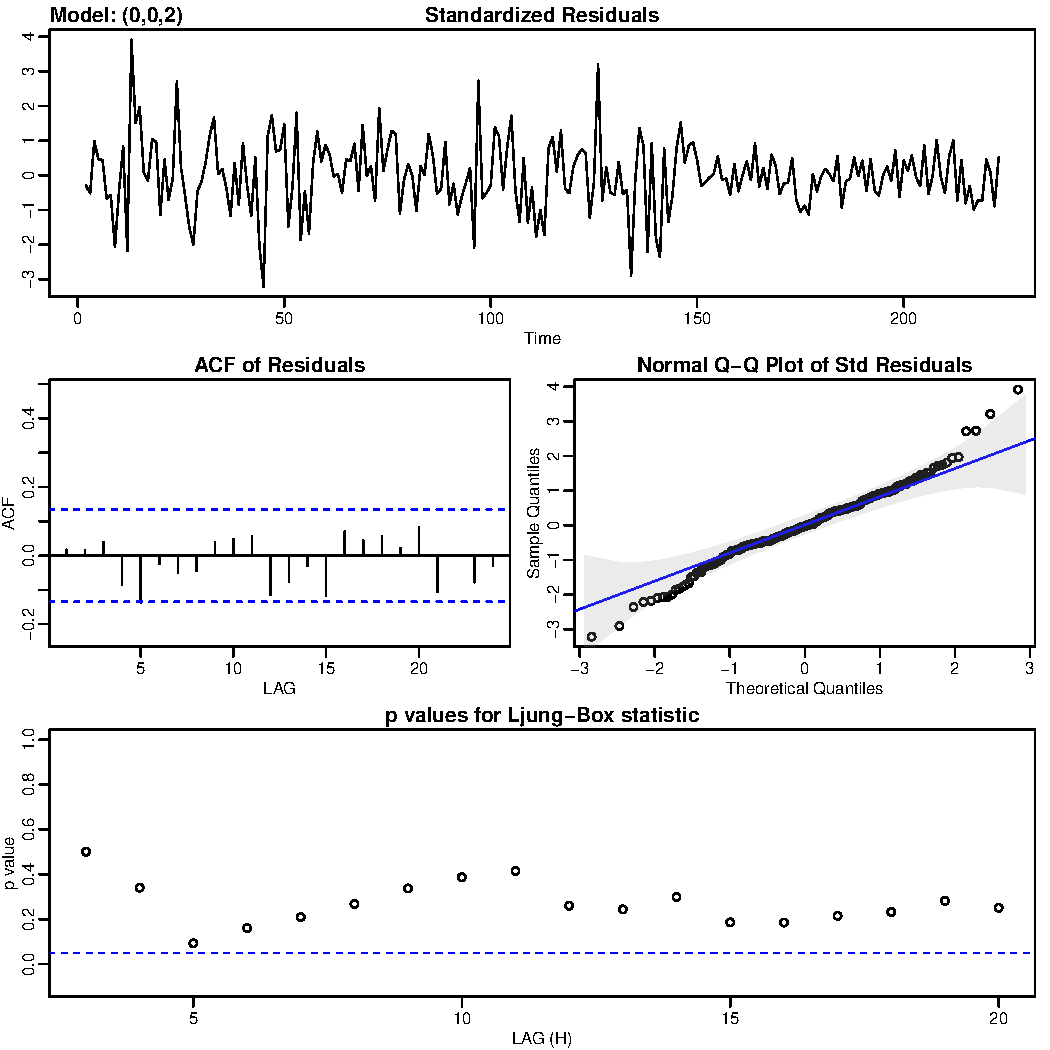
\includegraphics[width=100mm, height=60mm]{ma_diag.pdf}

Diagnostic plots for MA(2) model.

\end{frame}

\begin{frame}[fragile]
\frametitle{Worked Example: Model Selection}

AR(1) model.

\begin{verbatim}
sigma^2 estimated as 9.03e-05:

$AIC
[1] -6.44694

$AICc
[1] -6.446693

$BIC
[1] -6.400958
\end{verbatim}

\end{frame}

\begin{frame}[fragile]
\frametitle{Worked Example: Model Selection}

MA(2) model.

\begin{verbatim}
sigma^2 estimated as 8.919e-05

$AIC
[1] -6.450133

$AICc
[1] -6.449637

$BIC
[1] -6.388823
\end{verbatim}

\end{frame}

\begin{frame}[fragile]
\frametitle{Worked Example: ARMA Model}

How about an ARMA(2,2) model?

\begin{verbatim}
      Estimate     SE t.value p.value
ar1     1.3459 0.1374  9.7983  0.0000
ar2    -0.7378 0.1540 -4.7923  0.0000
ma1    -1.0634 0.1873 -5.6787  0.0000
ma2     0.5621 0.1971  2.8518  0.0048
xmean   0.0083 0.0008 10.4121  0.0000
\end{verbatim}

\end{frame}

\begin{frame}
\frametitle{Worked Example: Model Diagnostics}

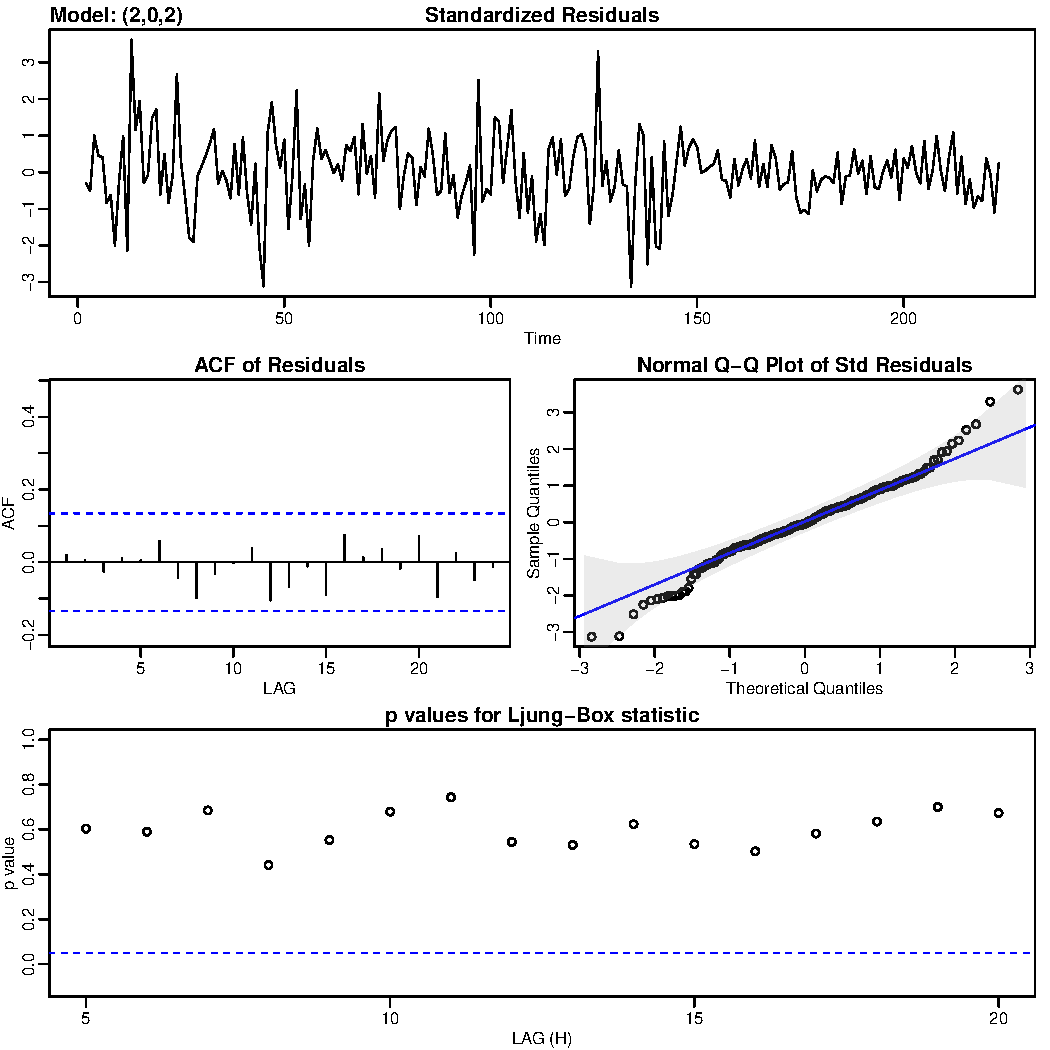
\includegraphics[width=100mm, height=60mm]{arma_diag.pdf}

Diagnostic plots for ARMA(2,2) model.

\end{frame}

\begin{frame}[fragile]
\frametitle{Worked Example: Model Selection}

ARMA(2,2) model.

\begin{verbatim}
sigma^2 estimated as 8.649e-05:

$AIC
[1] -6.462032

$AICc
[1] -6.46078

$BIC
[1] -6.370067

\end{verbatim}

\end{frame}

\begin{frame}[fragile]
\frametitle{Worked Example: Recap}

\begin{tabular}{c|c|c|c} % <-- Alignments: 1st column left, 2nd middle and 3rd right, with vertical lines in between
      & \textbf{AR(1)} & \textbf{MA(2)} & \textbf{ARMA(2,2)}\\
			\hline
      Est Coeffs& All significant & All significant & All significant\\
      Diagnostics & Ok & Ok & Ok\\
      AIC & -6.44694 & -6.450133 & \textbf{-6.462032}\\
			AICc & -6.446693 & -6.449637 & \textbf{-6.46078}\\
			BIC & \textbf{-6.400958} & -6.388823 & -6.370067\\
    \end{tabular}
		
\textbf{Question:} Which model will you choose? What else could be done to help us decide which model to choose?

\end{frame}

\begin{frame}
\frametitle{A Few More Comments about Model Building}

\begin{itemize}
\item Real data cannot be \textbf{exactly} modeled using a finite number of parameters.
\item What we want typically is a simple and accurate model.
\end{itemize}

\end{frame}

\end{document} 